\section{Experimental Evaluation}\label{sec:experiments}

In this section we present our experimental results in four parts.
\begin{enumerate}
    \item In Section~\ref{sec:eval_pddl+} we compare the performance of SMTPlan against other PDDL+ planners on PDDL+ benchmarks for hybrid systems domains. We aim to show that in problems with non-linear continuous change, and a small number of happenings, SMTPlan performs very well.
    
    \item In Section~\ref{sec:eval_objects} we investigate the scalability of SMTPlan in PDDL+ domains in more detail.
    
    \item In Section~\ref{sec:eval_pddl21} we compare SMTPlan with temporal planners from the International Planning Competition (IPC) on a set of temporal planning benchmarks used in the IPC. In the experiment we explore the limitations inherent in the Satisfiability approach in terms of scalability with respect to the size of the discrete state-space.
    
    \item Finally, in Section~\ref{sec:eval_cp} we evaluate the effect of control parameters on our encoding, comparing the effectiveness of SMTPlan on two versions of the same domain, with and without control parameters.
\end{enumerate}

\subsection{PDDL+ Benchmarks}\label{sec:eval_pddl+}

We use our encoding to solve PDDL+ planning problems with a parallel iterative deepening technique, widely used in SAT-based planning approaches~\cite{nab02,rin06}. The top-level algorithm encodes and solves $n$ SMT encodings simultaneously, solving the planning problem for horizon lengths $1,2,3,4,...,n$. In this case, horizon length corresponds to number of happenings. If a formula is found satisfiable, then a plan has been found and the planner terminates. If a formula is found unsatisfiable, then an encoding is made for the next shortest horizon length, so that there are always $n$ SMT instances being solved. The SMT solver we use is z3~\cite{dem08}.

We compare our approach (called SMTPlan) against existing PDDL+ planner UPMurphi~\cite{upmurphi}, and with dReach~\cite{bryce}, using the SMT solver dReal~\cite{gao12}, on domains both with and without events\footnote{We considered domains without events as we wanted to show the comparison with dReach which does not handle domains including events.}. We use the \textit{generator} and \textit{car} domains~\cite{bogomolov14}. The experiments were run using 8GB of RAM and a 30 minute timeout. All test domains and problems are available at: \textit{kcl-planning.github.io/SMTPlan}.

The generator domain is a PDDL+ benchmark problem that revolves around refueling a diesel-powered generator, which has to run for a given duration without overflowing or running dry. To test scalability the number of tanks is increased while decreasing the initial fuel level, so that all tanks are required.

We consider four versions of this domain: linear, simplified-nonlinear (the same used in~\cite{bryce}), nonlinear with events, and the Torricelli nonlinear~\cite{howey2003val}. Note that the latter version uses the Torricelli's Law, and hence the fuel level in a refueling tank ($V_{fuel}$) is calculated by:

\begingroup\makeatletter\def\f@size{10}\check@mathfonts
\begin{equation}
	V_{fuel} = (-kt_r+\sqrt[]{V_{init}})^2 \qquad t_r \in \left[0, \frac{\sqrt[]{V_{init}}}{k}\right] 
\end{equation}
\label{vol_eq}
\endgroup

where $V_{init}$ is the initial volume of fuel in the tank, $k$ is the fuel flow constant (which depends on gravity, size of the drain hole, and the cross-section of the tank), and $t_r$ is the time of refueling (bounded by the fuel level and the flow constant). An example of plan found by SMTPlan for the Torricelli nonlinear generator (Fuel level 960, Generator capacity 990) is shown in Figure~\ref{fig:generatorplan}:

\begin{figure}[htb!]
\centering
\small
\begin{BVerbatim}
0.0: generate     [1000.0]
959.0: refuel_tank1 [10.0]
959.0: refuel_tank2 [10.0]
\end{BVerbatim}
\caption{Plan for a problem in the Toricelli Generator domain.}
\label{fig:generatorplan}
\end{figure}

The car domain is another PDDL+ benchmark~\cite{pddl+} where a vehicle has to cover a given distance and have a zero velocity at the end, and the actions available are accelerate and decelerate that increments or decrements by 1 the current velocity, respectively.
To test scalability, the bound on maximum acceleration/deceleration is increased.

Our results for solvable instances are reported in Table~\ref{tab:solvable}. On both linear and nonlinear domains, SMTPlan outperforms all other planners in time to solve and in number of instances solved. In all domains, SMTPlan scales very well. For these domains, the number of happenings required is small, thus the minimal SMT encoding required to solve the problem is also small. The iterative deepening algorithm is able to reach a satisfiable encoding, and produce a plan very quickly. The offline computation with {\sc piranha} is required only once per domain, and in all cases requires 0.3 seconds or less.

dReach also performs iterative deepening, but performs more poorly. This is due to the semantics of dReach; in the dReach domain and problem description, each mode of continuous change must be explicitly defined, and the number of modes increases exponentially with the number of processes and durative actions (eg. the files for 1, 2, 3 and 4 tanks problems are respectively 91, 328, 1350, 5762 lines long). Furthermore, the bound is not on the number of happenings, but on the number of mode changes, which does not allow for parallel execution of actions. In contrast to SMTPlan, dReach does not perform integration and differentiation during encoding. Instead it relies upon the more expressive logic of the internal SMT solver, dReal. As a result, it is unable to use other SMT solvers.

We also compare our encoding directly against dReach as reported in prior work~\cite{bryce}: reporting times to solve only the encoding of a minimal step plan for each instance (Table~\ref{tab:finalstep}). These are not the times required to solve a PDDL+ instance, but a direct comparison of encodings on satisfiable problems. We find the encodings exhibit similar performance in the car domain. However, we find the SMTPlan encoding scales far better on the generator problem, for the reasons discussed above.

Our results for unsolvable instances are shown in Table~\ref{tab:unsolvable}. SMTPlan and dReach can only prove unsolvability up to an upper bound on the number of happenings. Here we prove plan non-existence for domains which have a tight deadline, and where each ground action can only be applied a finite number of times. We observe that both totally ordered planning approaches perform well proving unsolvability in the car domain. There are few choices of symbolic plan in this domain, leaving only the timing of the happenings and numeric constraints to be solved. Both SMTPlan and dReach solve these constraints very quickly. However, for PDDL+ problems in general, without deadlines and with repeatable actions, proving unsolvability is difficult through totally ordered planning with iterative deepening.

\begin{table*}[ht]
\centering
\def\arraystretch{1.2}
\begin{tabular}{|p{6em}|l|cccccccc|}
\hline
Domain         & Tool      & 1    & 2    & 3    & 4    & 5    & 6    & 7    & 8     \\
\hline
\multirow{3}{*}{\parbox{6em}{Generator linear}}
               & SMTPlan  & 0.02  & 0.03 & 0.02   & 0.01  & 0.02 & 0.02 & 0.02 & 0.02  \\
               & dReach    & 2.87  & -    & -      & -     & -    & -    & -    & -     \\
               & UPMurphi  & 0.2  & 18.2 & 402.34  & -     & -    & -    & -    & -     \\ % results from Bogolomov
\hline \hline
\multirow{3}{*}{\parbox{6em}{Generator nonlinear}}
               & SMTPlan  & 0.02  & 0.02 & 0.02   & 0.02  & 0.02  & 0.02  & 0.02    & 0.02   \\
               & dReach    & 5.16  & -    & -      & -     & -     & -     & -       & -      \\
               & UPMurphi  & 63.16 & -    & -      & -     & -     & -     & -       & -      \\
\hline \hline
\multirow{3}{*}{\parbox{6em}{Generator nonlin. events}}
               & SMTPlan  & 0.04 & 0.04 & 0.04 & 0.04  & 0.04 & 0.04 & 0.05 & 0.05  \\
               & dReach    & x    & x    & x    & x     & x    & x    & x    & x     \\
               & UPMurphi  & 658.18 & -    & -    & -     & -    & -    & -    & -     \\
\hline \hline
\multirow{3}{*}{\parbox{6em}{Generator Torricelli}}
               & SMTPlan  & 0.03  & 0.03 & 0.15 & 0.92  & 0.04 & 0.05 & 0.09 & 0.50  \\
               & dReach    & x     & x    & x    & x     & x    & x    & x    & x     \\
               & UPMurphi  & 63.16 & -    & -    & -     & -    & -    & -    & -     \\
\hline \hline
\multirow{3}{*}{\parbox{6em}{Car}}
               & SMTPlan  & 0.02  & 0.02  & 0.02 & 0.02  & 0.02 & 0.02 & 0.01 & 0.02  \\
               & dReach    & 1.30  & 1.41  & 1.48 & 1.53  & 1.47 & 1.54 & 1.40 & 1.53  \\
               & UPMurphi  & 28.44 & 386.5 & -    & -     & -    & -    & -    & -     \\ % results from Bogolomov
\hline
\end{tabular}
\caption{Results in seconds for solvable instances. Instance numbers correspond to number of tanks (generator) and number of acceleration steps (car). Abbrev.: ’-’: tool still running after 30 minutes, '.': tool ran out or memory, ’x’: tool cannot handle the problem.}
\label{tab:solvable}
\end{table*}

\begin{table*}[ht]
\centering
\def\arraystretch{1.1}
\begin{tabular}{|l|l|cccccccc|}
\hline
Domain         & Tool      & 1     & 2    & 3    & 4    & 5    & 6    & 7     & 8     \\
\hline

\multirow{2}{*}{\parbox{6em}{Generator linear}}
               & SMTPlan  & 0.00  & 0.01  & 0.01   & 0.01   & 0.01 & 0.02 & 0.02  & 0.02  \\
               & dReach    & 2.73  & 13.47 & 104.61 & 695.70 & -    & -    & -     & -     \\
\hline \hline
\multirow{2}{*}{\parbox{6em}{Generator nonlinear}}
               & SMTPlan  & 0.01  & 0.01    & 0.01 & 0.01   & 0.01 & 0.01 & 0.01  & 0.01 \\
               & dReach    & 10.42 & 1685.35 & -    & -      & -    & -    & -     & -    \\
\hline \hline
\multirow{2}{*}{\parbox{6em}{Car}}
               & SMTPlan  & 0.00  & 0.00 & 0.00 & 0.00 & 0.00 & 0.00 & 0.00 & 0.00  \\
               & dReach    & 0.77  & 0.76 & 0.76 & 0.76 & 0.76 & 0.76 & 0.77 & 0.76  \\
\hline
\end{tabular}
\caption{Results in seconds for minimal step encoding required to solve each instance.}
\label{tab:finalstep}
\end{table*}

\begin{table*}[ht]
\centering
\def\arraystretch{1.2}
\begin{tabular}{|l|l|cccccccc|}
\hline
Domain         & Tool      & 1    & 2      & 3     & 4    & 5      & 6    & 7    & 8     \\
\hline
\multirow{3}{*}{\parbox{6em}{Generator linear}}
               & SMTPlan & 0.01 & 0.02   & 0.16  & 2.84 & 390.86  & -    & -    & -     \\
               & dReach    & 2.57 & 189.94 & -     & -    & -      & -    & -    & -     \\
               & UPMurphi  & 0.90 & 29.42  & -     & -    & -      & -    & -    & -     \\ % results from Bogolomov
\hline \hline
\multirow{3}{*}{\parbox{6em}{Generator nonlinear}}
               & SMTPlan  & 0.01 & 1.95   & 33.48 & -    & -      & -    & -    & -     \\
               & dReach    & 2.43 & 212.43 & -     & -    & -      & -    & -    & -     \\
               & UPMurphi  & -    & -      & -     & -    & -      & -    & -    & -     \\
\hline \hline
\multirow{3}{*}{\parbox{6em}{Generator nonlin. events}}
               & SMTPlan  & 0.02   & 18.58   & 21.83 & -    & -      & -    & -    & -     \\
               & dReach    & x      & x       & x     & x    & x      & x    & x    & x     \\
               & UPMurphi  & -      & -       & -     & -    & -      & -    & -    & -     \\
\hline \hline
\multirow{3}{*}{\parbox{6em}{Generator Toricelli}}
               & SMTPlan  & 0.03  & 2.06   & 19.57 & -    & -      & -    & -    & -     \\
               & dReach    & x     & x      & x     & x    & x      & x    & x    & x     \\
               & UPMurphi  & -     & -      & -     & -    & -      & -    & -    & -     \\
\hline \hline
\multirow{3}{*}{\parbox{6em}{Car}}
               & SMTPlan  & 0.68  & 0.02   & 0.00  & 0.00 & 0.00   & 0.00 & 0.00 & 0.01  \\
               & dReach    & 0.67  & 0.50   & 0.62  & 0.45 & 0.58   & 0.57 & 0.49 & 0.65  \\
               & UPMurphi  & 36.01 & 445.23 & -     & -    & -      & -    & -    & -     \\ % results from Bogolomov
\hline
\end{tabular}
\caption{Results in seconds for unsolvable instances. Instance numbers correspond to number of tanks (generator) and number of acceleration steps (car). Abbrev.: ’-’: tool still running after 30 minutes, ’x’: tool cannot handle the problem.}
\label{tab:unsolvable}
\end{table*}

\subsection{Free Fall and Generator}\label{sec:eval_objects}

Two experiments were designed to explore the performance of SMTPlan on PDDL+ domains in more detail.

The first experiment evaluates the effects of having multiple objects in the domain file. The \textit{Free Fall} problem was extended, such that we consider problem instances where we have more than one ball. We considered two scenarios for these problem instances. In both scenarios we create cases that include 25, 50, 100, and 200 balls.
In the first scenario we try to find plans for the goal of catching just the first ball. As we increase the number of balls in the problem file, the search space grows exponentially. However, as shown in Figure~\ref{fig:Picture1}, the time needed to solve the problem increases only linearly. 
% (Any evidence for this?) SMTPlan focuses on variables related to the objects from the problem file that are involved in the goal state and tries to find the assignments for them. In other word, it also propagates the search branches regarding the variables that are representing other objects that are not in the goal state.
% (Really?) This means SMTPlan notices that the SMT variables related to the object that is in the goal state is the critical on and tries to solve them and propagate the other variables of the other objects. 
In the second scenario we continued the experiments by changing the goal state to catch all the balls in the problem file (we considered all the balls have the same initial height and we want to catch all of them at a certain height). Figure~\ref{fig:Picture1} shows the trend of the total time needed to solve the problem is linear in the number of balls. All the plans obtained from SMTPlan suggest to release all the balls together and also catch all of them at the same time point. This results from the fact that SMTPlan tries to solve the problem with minimum number of happenings.
% \footnote{As it is mentioned in Section~\ref{sssec:SMTPlan_Archi}, SMTPlan starts to find a plan with an initial number of happening which can be defined for it (otherwise it starts with two happening. If it can not find a plan it increases the number of happenings and this increase can be by one or a step size that can be defined for the planner. If we run the SMTPlan with the initial number of happenings of two and define that step size as one, the planner finds a planner with the minimum number of happenings, if the problem is solvable.}.  

These cases highlight that SMTPlan scales well with respect to the number of objects in the problem instance. While it is true that increasing the number of objects often will also increase the minimum number of required happenings, the iterative deepening search of SMTPlan will attempt to perform some parallelism of actions, if possible.

\iffalse
\begin{figure}[tbp!]
\centering
\begin{subfigure}[b]{0.48\textwidth}
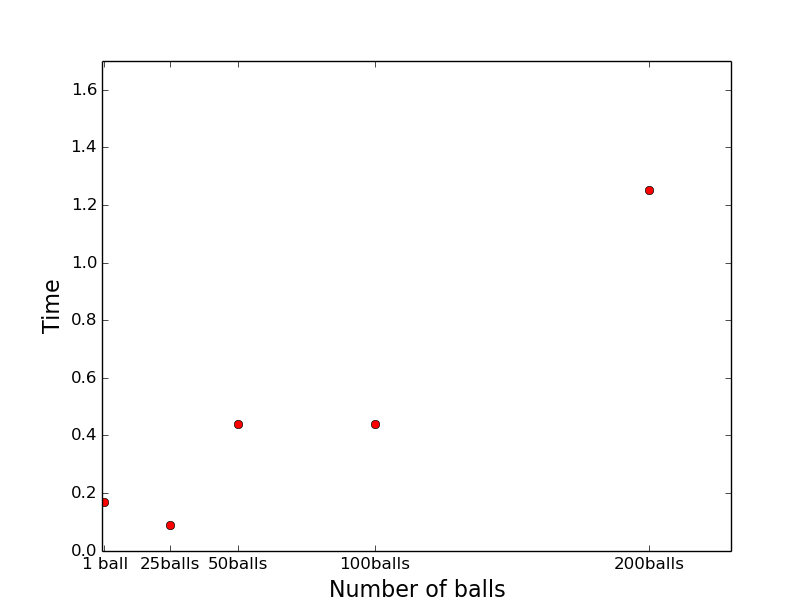
\includegraphics[width=\textwidth]{diagrams/Ball1.png}
\caption{Catch one ball}
\label{fig:Picture1}
\end{subfigure}
\hfill
\begin{subfigure}[b]{0.48\textwidth}
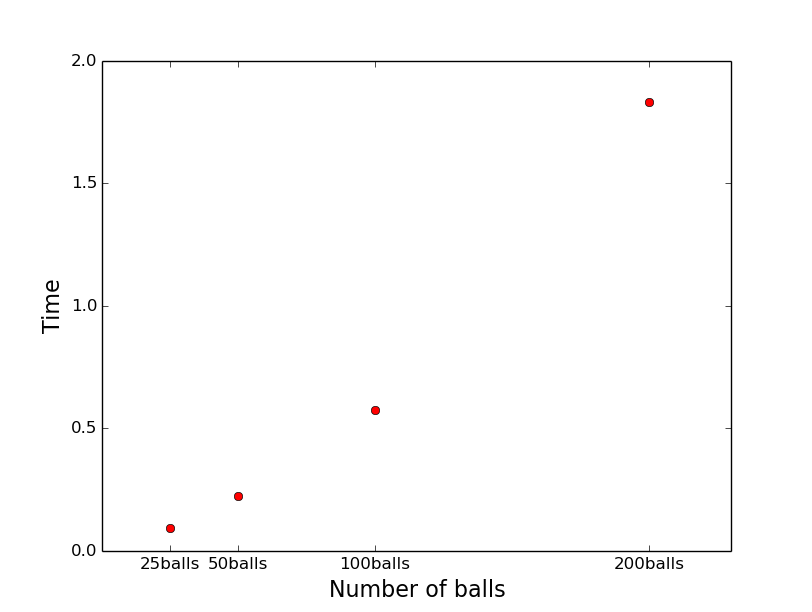
\includegraphics[width=\textwidth]{diagrams/Ball2.png}
\caption{Catch all the balls}
\label{fig:Picture2}
\end{subfigure}
\caption{(a):The Free Fall example with 1,25,50,100 and 200 balls. The goal is to catch the first bal.(b):The Free Fall example with 25,50,100 and 200 balls. The goal is to catch all the ball that have the same initial and goal state.}
\end{figure}
\fi

\begin{figure}[!ht]
\centering
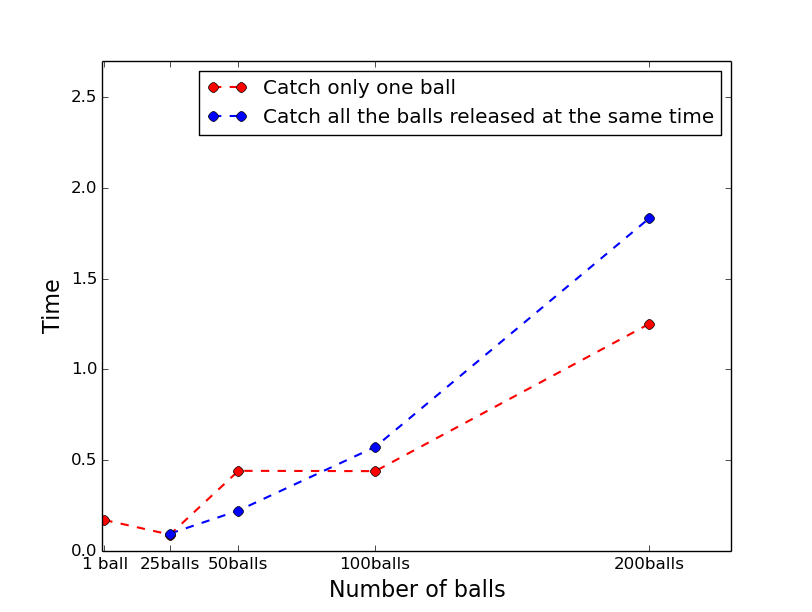
\includegraphics[width=0.70\textwidth]{diagrams/Balls.png}
\caption{The time taken (in seconds) for SMTPlan to solve the free fall problem with 1, 25, 50, 100 and 200 balls. The red line indicates the scenario in which and the aim of the problem is to just catch the first ball. The blue line represents the scenario with the goal is to catch all of them.}
\label{fig:Picture1}
\end{figure}

The second experiment tested the scaling performance of SMTPlan with respect to a longer time horizon. A number of problems were generated for the \textit{generator} domain in which the capacity and the running time of the generator increases gradually. In the benchmark problems the running time of the generator is $\num{1.000}$ time units. We created problems where the generator's running times has increased up to $\num{20.000}$ with increments of $\num{1.000}$ time units. To test the effects of the time horizon on the planner, we also changed the initial amount of the fuel in the tank, so that the number of times that we need to apply the re-fuelling action remains the same. In other words, just the length of the re-fuelling process has been extended.
The problems were solved with both SMTPlan and DiNo. 
As shown in Figures~\ref{fig:Picture4} and~\ref{fig:Picture3}, the time taken by SMTPlan to find a plan is not related to the time horizon. However, as we increase the time horizon, DiNo needs a longer time to solve the problem. As a forward search planner, the duration of the plan greatly impacts the performance of DiNo, and impacts the choice of discretisation that it can use. On the other hand, since the number of the happenings are the same, increasing the plan duration does not affect SMTPlan.

\begin{figure}[tbp!]
\centering
\begin{subfigure}[b]{0.49\textwidth}
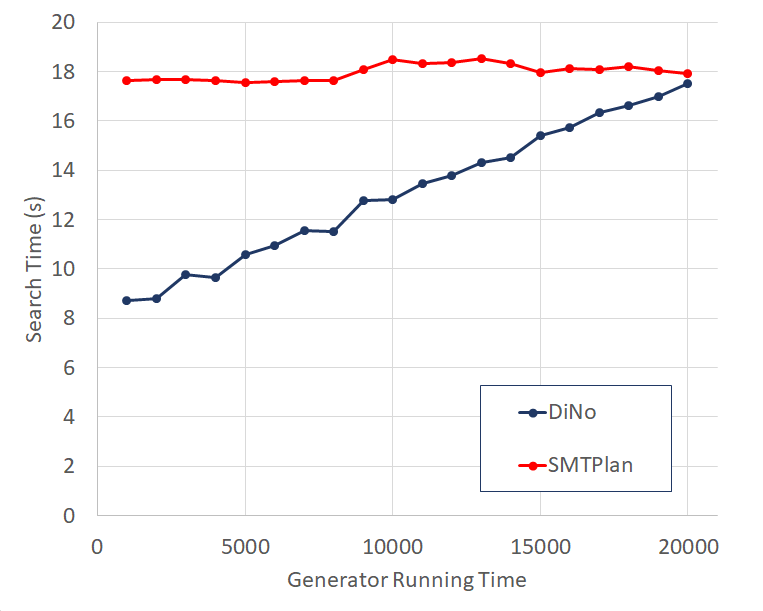
\includegraphics[width=0.99\textwidth]{diagrams/gen_event.png}
\caption{}
\label{fig:Picture4}
\end{subfigure}
\hfill
\begin{subfigure}[b]{0.48\textwidth}
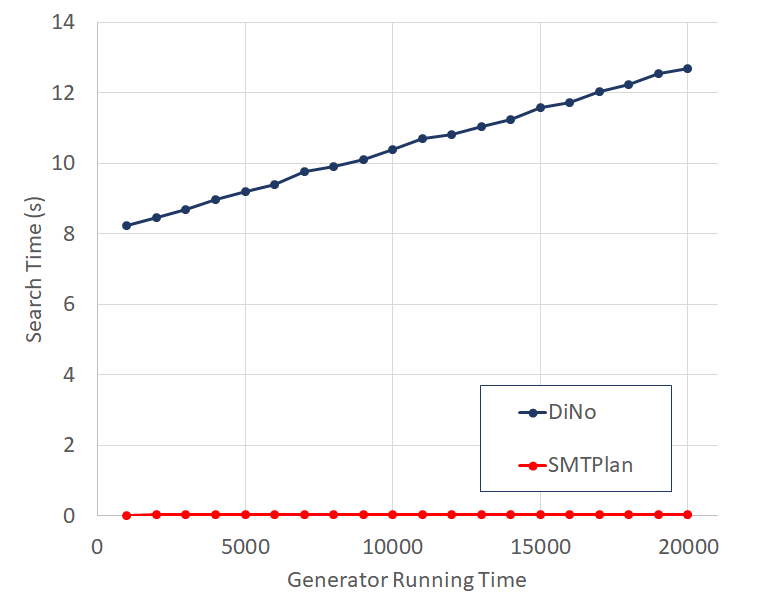
\includegraphics[width=0.99\textwidth]{diagrams/gen_linear.png}
\caption{}
\label{fig:Picture3}
\end{subfigure}
\caption{Generator domain with (a) nonlinear change and events and (b) only linear change, with increasing time horizon.}
\end{figure}

\iffalse
\begin{figure}[!ht]
\centering
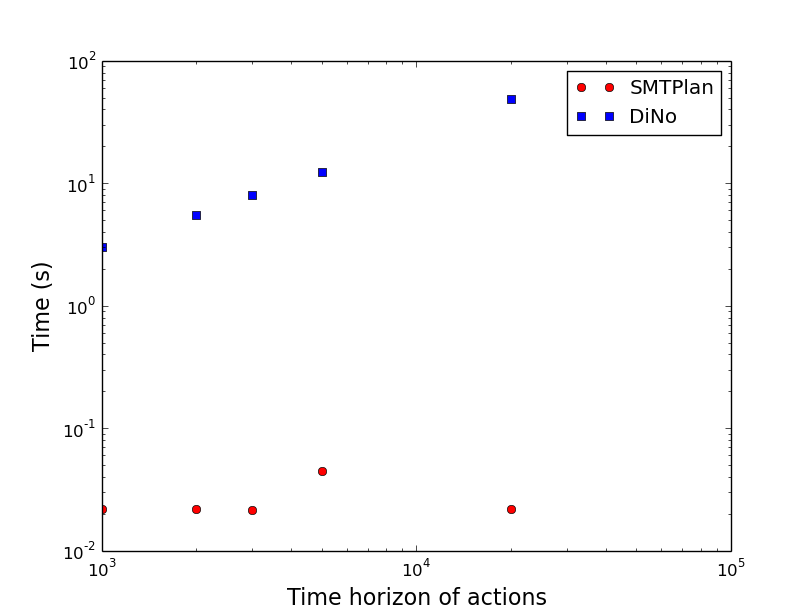
\includegraphics[width=0.80\textwidth]{diagrams/Generator_linear.png}
\caption{Generator domain with linear continuous changes with different time horizons}
\label{fig:Picture4}
\end{figure}
\fi
\subsection{Temporal Domains}\label{sec:eval_pddl21}

For the sake of completeness, and to investigate the scaling performance of SMTPlan with respect to the size of the discrete search space, we also tested the SMTPlan on the domains that were used in the temporal track of the International Planning Competition (IPC) at ICAPS 2018.
We compared the SMTPlan with the other planners participated in this track. These planners are CP4TP~\cite{cp4tp}, TFLAP~\cite{tflap}, TemPorAl~\cite{temporal}, PopCorn~\cite{popcorn} and OPTIC~\cite{OPTIC}. 
In total 10 domains were chosen. For each domain the first 10 problem instances were passed to the planner to solve. Each planner was given 30 minutes and 8GB of memory to solve as many problems as possible. The results are shown in Table~\ref{tab:ipc result}.
Each number in the table indicates the number of problem instances that each planner has managed to solve. In each row the largest number of problems for that domain solved by a single planner is shown in bold. 

As can be seen in the table, the performance gap between SMTPlan and temporal planners, on temporal planning problems, is large. While SMTPlan is highly effective on PDDL+ problems with nonlinear change and a small discrete search space, the large discrete search space for temporal planning problems is often insurmountable. One exception is the \textit{Cushing} domain, in which SMTPlan performed the best. This domain has a high degree of required concurrency, and can be difficult for other planning approaches, such as forward search. In addition, it allows for a great amount of parallelism of actions, therefore allowing SMTPlan to scale easily to all of the problem instances considered.


\begin{table}[thb]
\centering
\begin{tabular}{|l|l|l|l|l|l|l|l|}

\hline
                   &     & \multicolumn{6}{c|}{Planners}                                                 \\ \hline
Domain             & N   & SMTPlan     & CP4TP       & TFLAP       & TemPorAl    & PopCorn & OPTIC       \\ \hline
Airport            & 10  & 1           & 9           & 9           & \textbf{10} & 3       & 3           \\ \hline
Cushing            & 10  & \textbf{10} & \textbf{10} & 3           & 0           & 1       & \textbf{10} \\ \hline
Floortile          & 10  & 0           & 2           & 3           & \textbf{10} & 0       & 0           \\ \hline
Map Analyser       & 10  & 0            & \textbf{10} & 8           & \textbf{10} & 0       & 0           \\ \hline
Parking            & 10  & 0           & \textbf{10} & \textbf{10} & \textbf{10} & 4       & 8           \\ \hline
Quantum            & 10  & 1           & \textbf{10} & 8           & \textbf{10} & 5       & 8           \\ \hline
Road Traffic       & 10  & 0           & 7           & 0           & \textbf{10} & 0       & 0           \\ \hline
Sokoban            & 10  & 0           & \textbf{6}  & 4           & \textbf{6}  & 1       & 1           \\ \hline
Trucks-time-strips & 10  & 0           & \textbf{10} & \textbf{10} & \textbf{10} & 9       & \textbf{10} \\ \hline
Total              & 100 & 12          & 74          & 55          & \textbf{76} & 23      & 40          \\ \hline
\end{tabular}
\caption{Results in the number of problems that each planner could solve for the domains from ICAPS 2018 temporal tracks}
\label{tab:ipc result}
\end{table}

\subsection{Domains with Control Parameters}\label{sec:eval_cp}

In this section we have designed a set of experiments to show how introducing control parameters affects the performance of SMTPlan. We used the \textit{cashpoint} domain for these experiments, solving problems with SMTPlan on two different variants of the domain: one including control parameter variables and the other one without. Similarly to Savas et al.~\cite{savas2016planning}, in the domain without control parameters we add a number of \textit{withdraw\_money} actions with fixed withdrawal values, namely $\{1, 5, 10, 20\}$. For both domains we considered a set of problem instances that get more difficult gradually. Six sets of problem instances were generated with an increasing number of bank locations (from 1 to 6). In each problem every bank must be visited to achieve the goal. Problems within each set increase in difficulty due to additional locations and goals.

The results for these experiments are shown in Table~\ref{tab:table_results_cp} and Figure~\ref{fig:CP_results}. Table~\ref{tab:table_results_cp} shows the number of problems that could be solved with and without control parameters. By using control parameters, repeated applications of the same action can be avoided, lowering the number of required happenings. This allows SMTPlan to solve many more problems.

Figure~\ref{fig:CP_results} compares the time taken to solve problems that were solved both with and without control parameters. As we can see on the graph, the time to solve the problems without control parameters is generally much longer. However, in smaller problems the overhead of introducing the control parameter variables and constraints leads to longer solution times.

\begin{figure}[!ht]
\centering
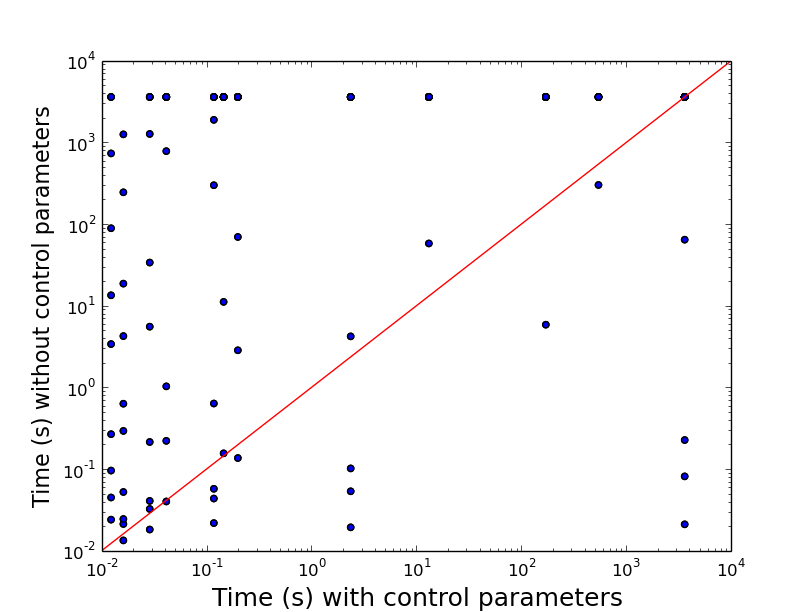
\includegraphics[width=0.60\textwidth]{diagrams/CP_results.png}
\caption{Comparison of time taken to solve problems in the \textit{cashpoint} domain with and without control parameters.}
\label{fig:CP_results}
\end{figure}



% Please add the following required packages to your document preamble:
% \usepackage{multirow}
\begin{table}[!ht]
\centering
\begin{tabular}{|c|c|c|c|}
\hline
\multirow{2}{*}{\begin{tabular}[c]{@{}c@{}}No. \\ Banks\end{tabular}} & \multirow{2}{*}{\begin{tabular}[c]{@{}c@{}}Total \\ Problems\end{tabular}} & \multicolumn{2}{c|}{\begin{tabular}[c]{@{}c@{}}Problems \\ Solved\end{tabular}} \\ \cline{3-4} 
                                                                      &                                                                            & \multicolumn{1}{l|}{With CP}          & \multicolumn{1}{l|}{Without CP}         \\ \hline
1                                                                     & 60                                                                         & 40                                    & 16                                      \\ \hline
2                                                                     & 60                                                                         & 30                                    & 13                                      \\ \hline
3                                                                     & 60                                                                         & 20                                    & 8                                       \\ \hline
4                                                                     & 60                                                                         & 10                                    & 6                                       \\ \hline
5                                                                     & 60                                                                         & 10                                    & 4                                       \\ \hline
6                                                                     & 60                                                                         & 0                                     & 0                                       \\ \hline
\end{tabular}
\caption{Comparison of number of problems that can be solved by SMTPlan with and without control parameters.}
\label{tab:table_results_cp}
\end{table}


